% Article type supporting font formatting
\documentclass[a4paper,12pt]{extarticle}

% Define .tex file encoding
\usepackage[utf8]{inputenc}

% Norwegian language support
%\usepackage[norsk]{babel}     

% Indent first paragraph in section
\usepackage{indentfirst}

% Allows mathbb in tex file
\usepackage{amsfonts} 

\usepackage{lmodern,textcomp}

% Margin defining package
\usepackage{geometry}         
\geometry{a4paper
  ,margin=1in
}

% For quotations
\usepackage{csquotes}

% Better bibliography 
\usepackage[square,numbers]{natbib}

% For use of graphics in document
\usepackage{graphicx}         

% Allows multi-line comments in tex file
\usepackage{verbatim}         

% Allows math in tex file 
\usepackage{amsmath}          

% Allows math symbols in tex file
\usepackage{amssymb}          

% Allows use of physics shortcut functions
%\usepackage{physics}          

% Verbatim env with LaTeX commands
\usepackage{alltt}            

% Allows \begin{figure}[H]
\usepackage{float}

% Adds labeling list to the report
\usepackage{scrextend}
\addtokomafont{labelinglabel}{\ttfamily}

% Necessary for defining colours
\usepackage{xcolor}            
\definecolor{linkgreen}{rgb}{0,.5,0}
\definecolor{linkblue}{rgb}{0,0,.5}
\definecolor{linkred}{rgb}{.5,0,0}
\definecolor{blue}{rgb}{.13,.13,1}
\definecolor{green}{rgb}{0,.5,0}
\definecolor{red}{rgb}{.9,0,0}

% Hyperlinks in document
\usepackage{hyperref}  
\hypersetup{
  colorlinks=true,     % True for colored links
  linktoc=all,         % True for table of contents links
  linkcolor=linkblue,  % Colour for links
  urlcolor=linkgreen,  % Colour for URLs
  citecolor=linkred    % Colour for citations
}

% Listing package for code examples
\usepackage{listings}         
\lstset{
  language=C++,                % Set language to C++
  showspaces=false,            % Don't show space chars
  showtabs=false,              % Don't show tab chars
  breaklines=true,             % Break long lines of code
  showstringspaces=false,      % Don't show spaces in strings
  breakatwhitespace=true,      % Break at white space only
  commentstyle=\color{green},  % Set colour for comments
  keywordstyle=\color{blue},   % Set colours for keywords
  stringstyle=\color{red},     % Set colour for strings
  basicstyle=\ttfamily,        % Set basic style
  tabsize=2                    % Set tabsize
}

% Referencing, last for compatibility reasons
\usepackage[noabbrev]{cleveref}

% Command to set two lines under text
\newcommand{\uunderline}[1]{\underline{\underline{#1}}}

% Command to use integral with limits
\newcommand{\Int}{\int\limits}    

% Command to use double integral with limits
\newcommand{\IInt}{\iint\limits}  

% Command to use triple integral with limits
\newcommand{\IIInt}{\iiint\limits}

% Command removes section numbering
\newcommand{\mysection}[2]{   
  \setcounter{section}{#1}
  \section*{#2}
  \addcontentsline{toc}{section}{#2}
}

% Command removes subsection numbering
\newcommand{\mysubsection}[2]{  
  \setcounter{subsection}{#1}
  \subsection*{#2}
  \addcontentsline{toc}{subsection}{#2}
}

% Command removes subsubsection numbering
\newcommand{\mysubsubsection}[2]{ 
  \setcounter{subsubsection}{#1}
  \subsubsection*{#2}
  \addcontentsline{toc}{subsubsection}{#2}
}

% Makes matrices look square-ish
\renewcommand*{\arraystretch}{1.5}

\usepackage{tikz}

\newcommand{\shrug}[1][]{%
  \begin{tikzpicture}[baseline,x=0.8\ht\strutbox,y=0.8\ht\strutbox,line width=0.125ex,#1]
  \def\arm{(-2.5,0.95) to (-2,0.95) (-1.9,1) to (-1.5,0) (-1.35,0) to (-0.8,0)};
  \draw \arm;
  \draw[xscale=-1] \arm;
  \def\headpart{(0.6,0) arc[start angle=-40, end angle=40,x radius=0.6,y radius=0.8]};
  \draw \headpart;
  \draw[xscale=-1] \headpart;
  \def\eye{(-0.075,0.15) .. controls (0.02,0) .. (0.075,-0.15)};
  \draw[shift={(-0.3,0.8)}] \eye;
  \draw[shift={(0,0.85)}] \eye;
  % draw mouth
  \draw (-0.1,0.2) to [out=15,in=-100] (0.4,0.95); 
  \end{tikzpicture}}

%%%%%%%%%%%%%%%%%%%%%%%%%%%%%%%%%%%%%%%
%%      Title, Author, and Date      %%
%%%%%%%%%%%%%%%%%%%%%%%%%%%%%%%%%%%%%%%
\title{Visualizing Terrain Data through Ray Tracing}
\author{Daniel Aaron Salwerowicz, Christopher Kragebøl Hagerup}
\date{\today}
%%%%%%%%%%%%%%%%%%%%%%%%%%%%%%%%%%%%%%%
%%           Start document          %%
%%%%%%%%%%%%%%%%%%%%%%%%%%%%%%%%%%%%%%%
\begin{document}
  
%%%%%%%%%%%%%%%%%%%%%%%%%%%%%%%%%%%%%%%
%%   Create the main title section   %%
%%%%%%%%%%%%%%%%%%%%%%%%%%%%%%%%%%%%%%%
\maketitle

%%%%%%%%%%%%%%%%%%%%%%%%%%%%%%%%%%%%%%%
%%      Abstract for the report      %%
%%%%%%%%%%%%%%%%%%%%%%%%%%%%%%%%%%%%%%%
% \begin{abstract} 
% Say why this report exists. Motivations behind it and what not.
% \end{abstract}

%%%%%%%%%%%%%%%%%%%%%%%%%%%%%%%%%%%%%%%
%%         ToC for the report        %%
%%%%%%%%%%%%%%%%%%%%%%%%%%%%%%%%%%%%%%%
% \tableofcontents
% \pagebreak

%%%%%%%%%%%%%%%%%%%%%%%%%%%%%%%%%%%%%%
%%  The main content of the report  %%
%%%%%%%%%%%%%%%%%%%%%%%%%%%%%%%%%%%%%%
\mysection{1}{Introduction}
Our goal in this project was to use raycasting to visualize terrain data of Bjerkvik in a 3D-space. The data was provided in the form of a text file with points, and our aim was to see if we could use colors to visualize different parameters in the 3D-model. Examples of parameters that we could use were \emph{height} and \emph{point density}.
%In this project we aimed to visualize intrinsic properties of B-Spline curves (curve from now on) in 3D-space. These intrinsic curve properties are \emph{curvature} and \emph{torsion}. Curvature defines how fast a curve changes direction at any given point, whereas torsion defines how much the curve is "twisting" or "coming out of" the plane of curvature. As such we see that a curve cannot have torsion at a point if there is no curvature there. \cite{jia_2017}

\mysection{2}{Methods}
%TODO: Check if this is actual bullshit or not, was really tired when I wrote this.
We used GMlib to represent and render the terrain in 3D-space, and used a technique called ray casting to render the terrain to the window.

In our application, data is first read from a file. After all of the samples have been stored in the file, we determine the maximum and minimum values in the x-, y- (and z?)-axis. After we have found these values, we use them to normalize all of the data to our space, where we partition the volume into samples, and determine the amount of points in each sample. This amount is used to determine the color and alpha (transparency) of the sample.

Sans and Ramona \cite{san_2017} defines ray casting as a technique for rendering three-dimensional shapes without having to reconstruct the data. For each pixel in the image, a ray is cast into the canvas, and the models in the picture are visualized by having the light interact with the samples from the data. Unlike the similarly named ray-tracing, ray casting does not trace rays recursively, and instead only does it once. The benefit of using ray casting is that the work is light and can easily be panellised, making it ideal for a Graphics-Processing Unit (GPU).

We also make use of a transfer function in our code. A transfer function is a function that determines the color of the different samples in the model based on one or more parameters. In our case, the transfer function highlights the point density. In addition, the transfer function is vital for making sure that the volume is displayed correctly, as the shape will not be mapped properly without it.
%We have used GMlib to represent a curve in 3D space as well as representing its curvature using ovals (circles) and torsion using colours. 

%To represent curvature we transform the curvature measured with vector into a circle with radius equal length of the vector. Curvature at a given point is calculated using:
%\begin{align*}
%  \kappa(t) = \frac{\left\|c^{'}(t) \times c^{''}(t)\right\|}{\left\|c^{'''}(t)\right\|^3}
%\end{align*}
%As such these circles easily and intuitively convey the curvature of curve at any given point and how it changes over its length.

%Torsion is represented with colours in HSV colour model, where hue is decided by the sign of torsion and saturation is decided by relative strength of torsion. Torsion itself is calculated by: 
%\begin{align*}
%  \tau(t) = \frac{\left(c^{'}(t) \times c^{''}(t) \right)\cdot c^{'''}(t)}{\left\|c^{'}(t) \times c^{''}(t)\right\|^2}
%\end{align*}
%As such torsion is conveyed using colours and intesity to show its magnitude.

%Here we will explain what we do to visualize these properties. First we create a \verb|MyBSplineCurve| object that then creates a \verb|MyVisualizer| instance and it in turn creates \verb|CurveParam| objects that hold values relevant for visualization (see \cref{fig:uml}). These structs hold one \verb|PCircle| that they are responsible for visualizing and updating. Each time the curve is changed it calls on updateParams method which in turn moves and updates circles.
%\begin{figure}[H]
%  \centering
%  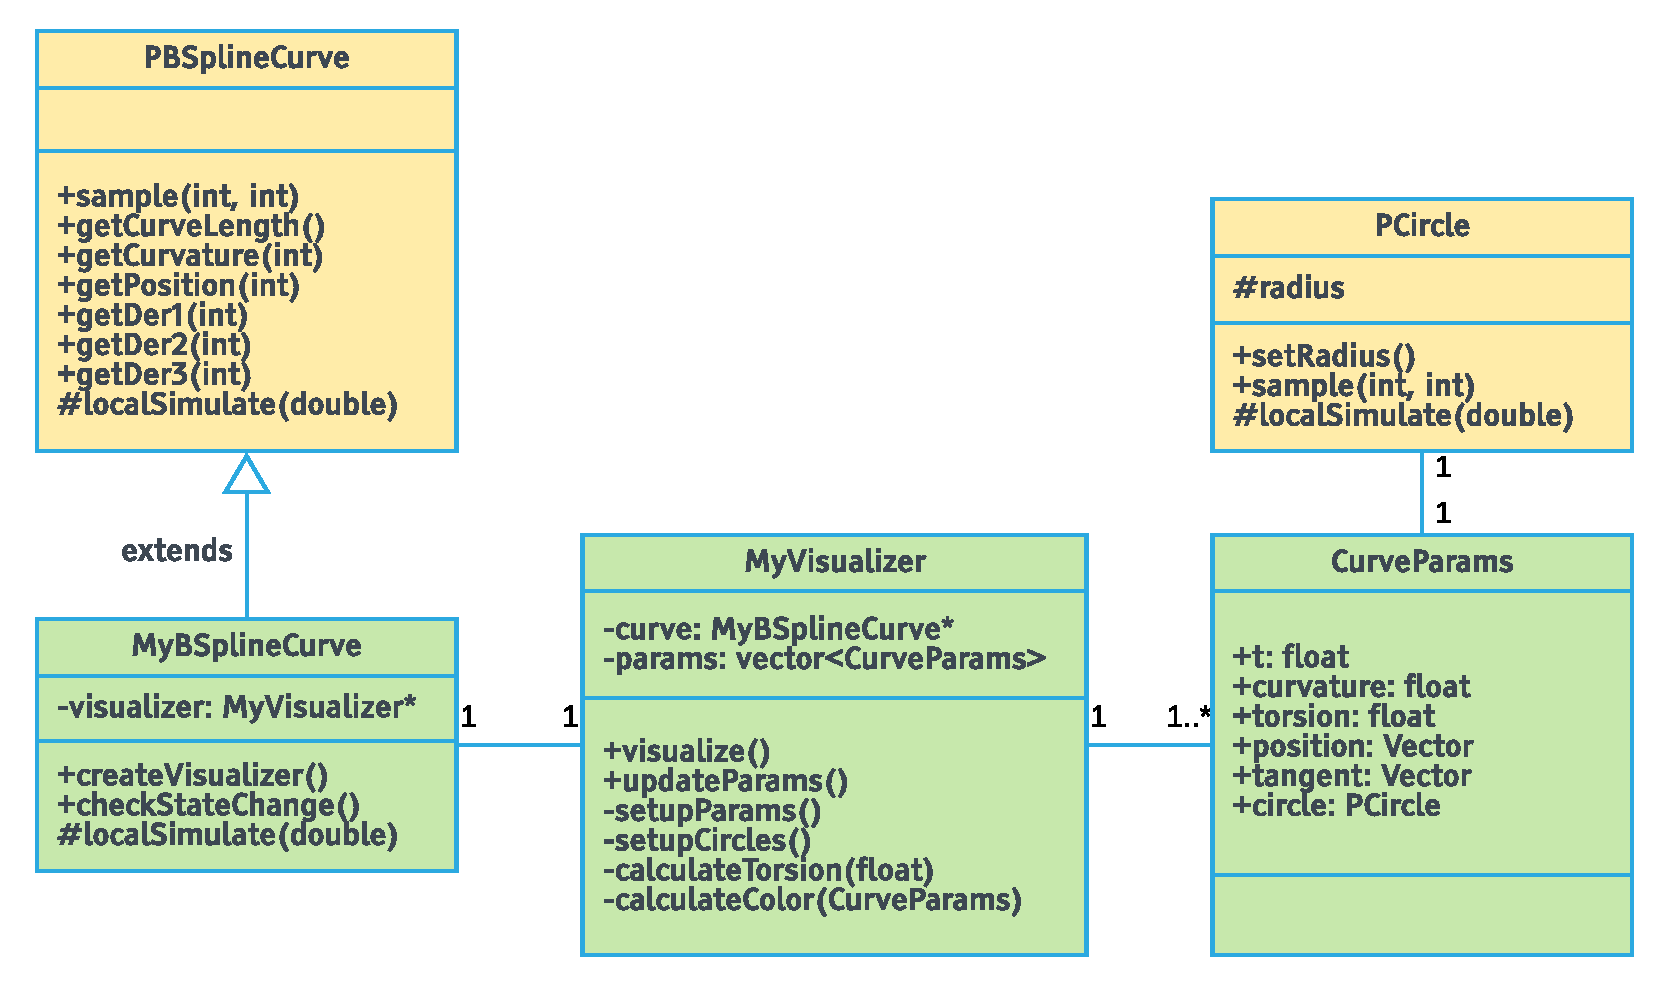
\includegraphics[width=\textwidth]{KurwatureUML}
%  \caption{UML class diagram our program.}
%  \label{fig:uml}
%\end{figure}

\mysection{3}{Results}
Our result is a program where you can see the terrain visualized. The visualization can be rotated and viewed from different angles, and you can easily make out the terrain (Even though it is a bit stretched at the moment). On one of the sides of the GUI (right or left), there are four coloured boxes, which provide the colour points for the transfer function. Clicking on the boxes adds a point with the colour clicked to the transfer function, and you can click a box multiple times to add different gradients of a colour
%We have ended up with a really adequate visualization program for curvature and torsion where user can easily see both of these properties. Visualization is really easy to inspect, transform and see how curvature and torsion change after manipulation. \Cref{fig:kurwature} shows an example of curve simulated and visualized in our program. User can easily twist, bend and rotate the curve to inspect how distorions of it change its properties.
%\begin{figure}[H]
%  \centering
%  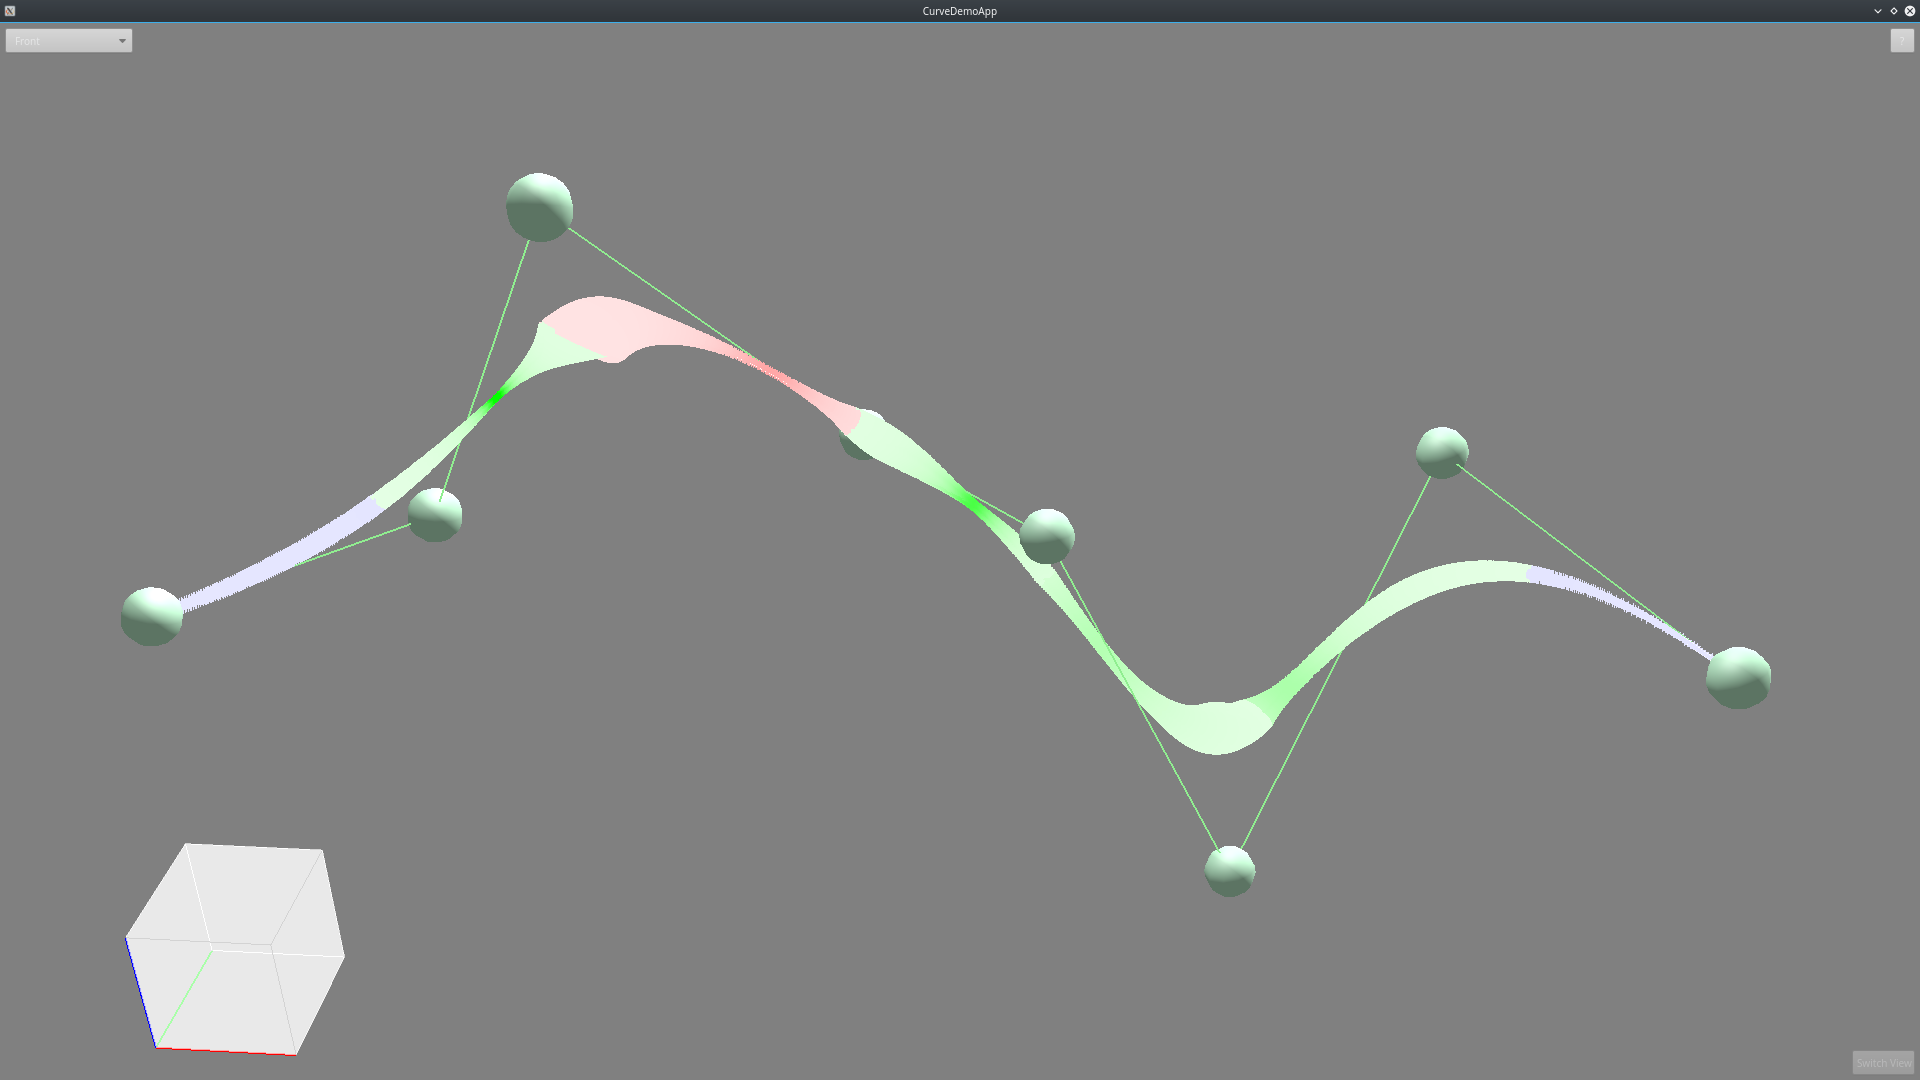
\includegraphics[width=0.8\textwidth]{Kurwature}
%  \caption{Visualization of curvature and torsion in our program.}
%  \label{fig:kurwature}
%\end{figure}

\mysection{4}{Analysis}
%Based on our calculations and observations we conclude that this visualization program is quite accurate and represents the curve properties quite well. We have found out that in some instances it could've been beneficial to normalize the curvature values as to limit how big the circles can grow, but in most usecases this proved to be unnecessary, and it could easily be avoided by setting limitations on curve editing capabilities. 

%We have tried many different ways of displaying torsion by, but after discussion with Børre Bang we came to conclusion that this is the most readable option for displaying torsion. So hue is set by torsions sign, and saturation is set by relative value of torsion. Saturation is given by:

%\begin{align*}
%  saturation=\frac{|\tau|}{|\tau_{max}|}
%\end{align*}
%which will normalize the torsion values so that both negative and positive torsion values are set based on maximum torsion.

\mysection{5}{Discussion}
%We are quite happy with our visualizer, it is quite simple and easy to understand as well as it is lightweight and does not require use of shaders. It runs quite fast and lets user easily understand what he sees on the screen. It is also dynamic so each small edit made to curve is immediatly displayed on screen.

%There are of course possibilities for further development and improvements in our visualizer. One of these would be to implement restrictions on curve editing, so we don't end up with enourmous circles that result from extremely high curvature. Another feature worth implementing would be possibility to visualize higher order derivatives of curve, that could be easily done by adding lines at various points in curve with length equal to magnitude of these derivatives.

\mysection{6}{Bibliography}
\begingroup
\def\section*#1{}
\bibliographystyle{apa}
\bibliography{Bibliography}
\endgroup

\end{document}
